% !TeX root = ../main.tex
\section{Computational cost}
\label{sec:scalability}

% ===========================================================================
% Evidence: experiments/scalability/ (timings.csv, table_cost_scaling_body.tex, make_cost_figure.py; rewritten 2026-10-01 for the exact augmented sampler).
%   run_config.R        one (method, n, replicate) per R process, both samplers' own source files with clock reads only
%   run_timing*.sh      sequential drivers;  results/raw/*.rds, results/timing_log.txt
%   profile_mvrnorm.R   dense operations of the Onizuka theta draw in isolation -> results/mvrnorm_profile.csv
%   collect.R, analyze.py -> results/numbers.json, results/table_time_body.tex, figures/scal_*.pdf (copied to figures/)
% Every number below is taken from results/numbers.json, table_time_body.tex or mvrnorm_profile.csv.
% 2026-10-02: wall-time-per-run material removed; the section reports time per sweep and its breakdown only.
% Previous versions of this section: notes/scalability_rewrite_20261001/before/scalability.tex.
% ===========================================================================

We compare the time per Gibbs sweep of Bayesian-PMALA with that of the Laplace and horseshoe samplers of \citet{onizuka2024fast}. All three use the same augmentation and differ in the trend update. Bayesian-PMALA computes two proximal maps by ADMM with a fixed iteration budget and banded factorizations (Section~\ref{subsec:pmala}), so its sweep costs $O(n)$. The supplied Onizuka code draws the trend from its Gaussian full conditional by forming the dense inverse of the precision matrix and an eigendecomposition (\texttt{MASS::mvrnorm}), whose cost grows cubically in $n$.

\paragraph{Protocol.} We use the VS signal \eqref{eq:sim_vs} with Gaussian noise, $\tau = 0.5$, $k = 2$ and $n$ from $250$ to $4000$, with the same data for all samplers. The Onizuka code is unmodified, with \texttt{sparse = TRUE}, and both samplers are timed by clock reads around their updates. All runs use one laptop core (Intel Core Ultra 7 155U, R~4.4.1, reference BLAS). Warm-up and setup are excluded, and each entry is the median over up to three replicates with distinct data.

\begin{table}[!htbp]
\centering
\footnotesize
\caption{Time per Gibbs sweep in milliseconds: median over replicates, with the range below ($\dagger$: single replicate). Ratios divide the median Onizuka time by the median Bayesian-PMALA time.}
\label{tab:cost_scaling}
\begin{tabular}{rrrrrr}
\toprule
 & \multicolumn{3}{c}{Time per sweep (ms)} & \multicolumn{2}{c}{Ratio to PMALA} \\
\cmidrule(lr){2-4}\cmidrule(lr){5-6}
$n$ & PMALA & Laplace & Horseshoe & Laplace & Horseshoe \\
\midrule
250 & 2.0 & 48.4 & 47.2 & 25 & 24 \\
 & (1.9--2.8) & (42.4--52.6) & (37.7--72.1) & & \\
\addlinespace
500 & 4.2 & 314 & 318 & 75 & 76 \\
 & (3.6--4.9) & (246--401) & (265--329) & & \\
\addlinespace
1\,000 & 9.2 & 3\,650 & 2\,918 & 398 & 318 \\
 & (6.7--12.0) & (1\,840--4\,648) & (2\,183--3\,657) & & \\
\addlinespace
2\,000 & 16.1 & 21\,857 & 32\,543 & 1\,360 & 2\,025 \\
 & (15.7--23.8) & (20\,633--23\,081) & (22\,905--42\,180) & & \\
\addlinespace
4\,000 & 36.6 & 257\,660 & 241\,459 & 7\,035 & 6\,593 \\
 & (26.7--38.1) & $^{\dagger}$ & $^{\dagger}$ & & \\
\bottomrule
\end{tabular}
\end{table}

\begin{figure}[!htbp]
\centering
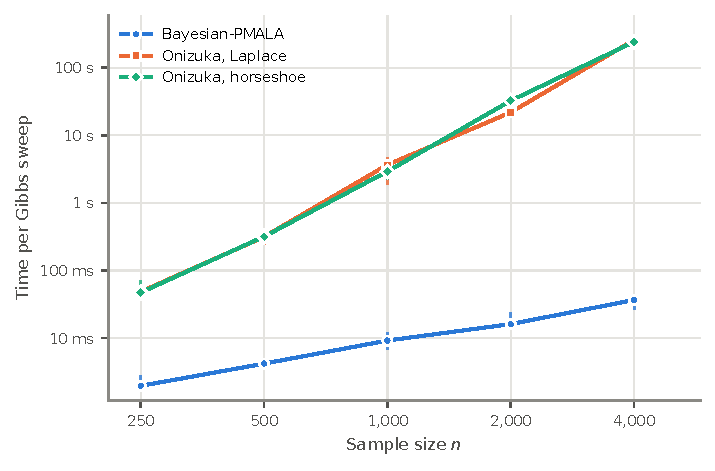
\includegraphics[width=0.7\textwidth]{figures/scal_time.pdf}
\caption{Median time per Gibbs sweep against $n$ (log--log), with bars spanning the range across replicates.}
\label{fig:cost_scaling}
\end{figure}

\paragraph{Results.} The time per sweep of Bayesian-PMALA grows linearly with $n$, at an essentially constant cost per observation, whereas an Onizuka sweep grows roughly cubically, so the gap widens with every doubling of $n$, from about one order of magnitude at the smallest $n$ to nearly four at the largest (Table~\ref{tab:cost_scaling}, Figure~\ref{fig:cost_scaling}). The two Onizuka priors cost the same. Almost all of a Bayesian-PMALA sweep is the P-MALA move, and almost all of an Onizuka sweep is the dense inverse and eigendecomposition of the trend draw (Figure~\ref{fig:cost_breakdown}).

The gap belongs to the supplied implementation rather than to the horseshoe hierarchy, whose precision matrix is banded and admits a banded Cholesky draw. The comparison concerns time per sweep, not the efficiency of the chains per sweep.

\begin{figure}[!htbp]
\centering
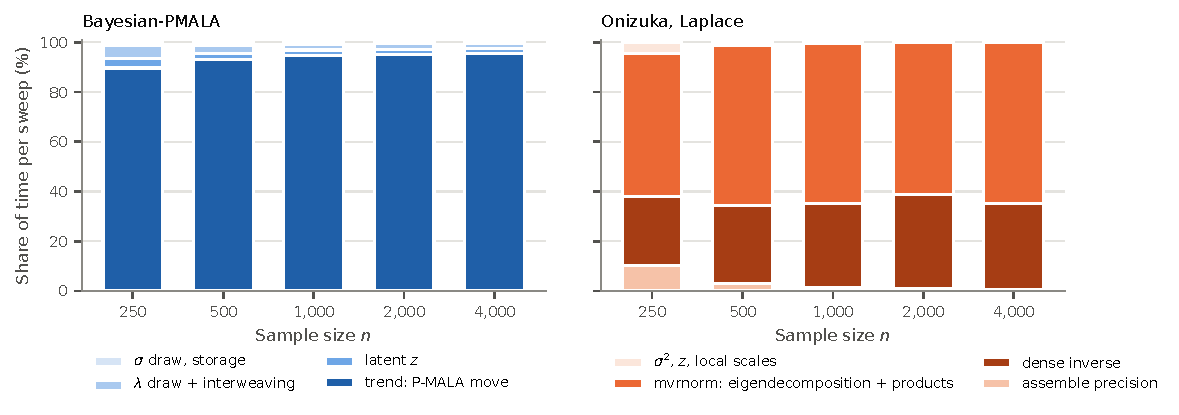
\includegraphics[width=\textwidth]{figures/scal_breakdown.pdf}
\caption{Share of the time per sweep spent in each update (median over replicates). Left: Bayesian-PMALA. Right: the Onizuka Laplace sampler; the horseshoe sampler's shares agree to within three percentage points.}
\label{fig:cost_breakdown}
\end{figure}
